In the last section, we have developed a formal language for representing multigrid methods with the use of simple state transition functions.
Furthermore, we have shown how it is possible to formulate a context-free grammar for generating representations of arbitrarily-structured multigrid methods in that language.
As we have already discussed in this section, due to the context-independence of each production of this grammar, each of its derivations can be formulated as a tree.
For this purpose, consider again the three-grid method shown in Algorithm~\ref{alg:example-three-grid-method}.
We can now express this method as a sequence of the productions defined in Section~\ref{sec:multigrid-grammar}, which leads to the derivation tree shown in Figure~\ref{fig:example-three-grid-method-derivation-tree}.
\begin{figure}
	\centering
	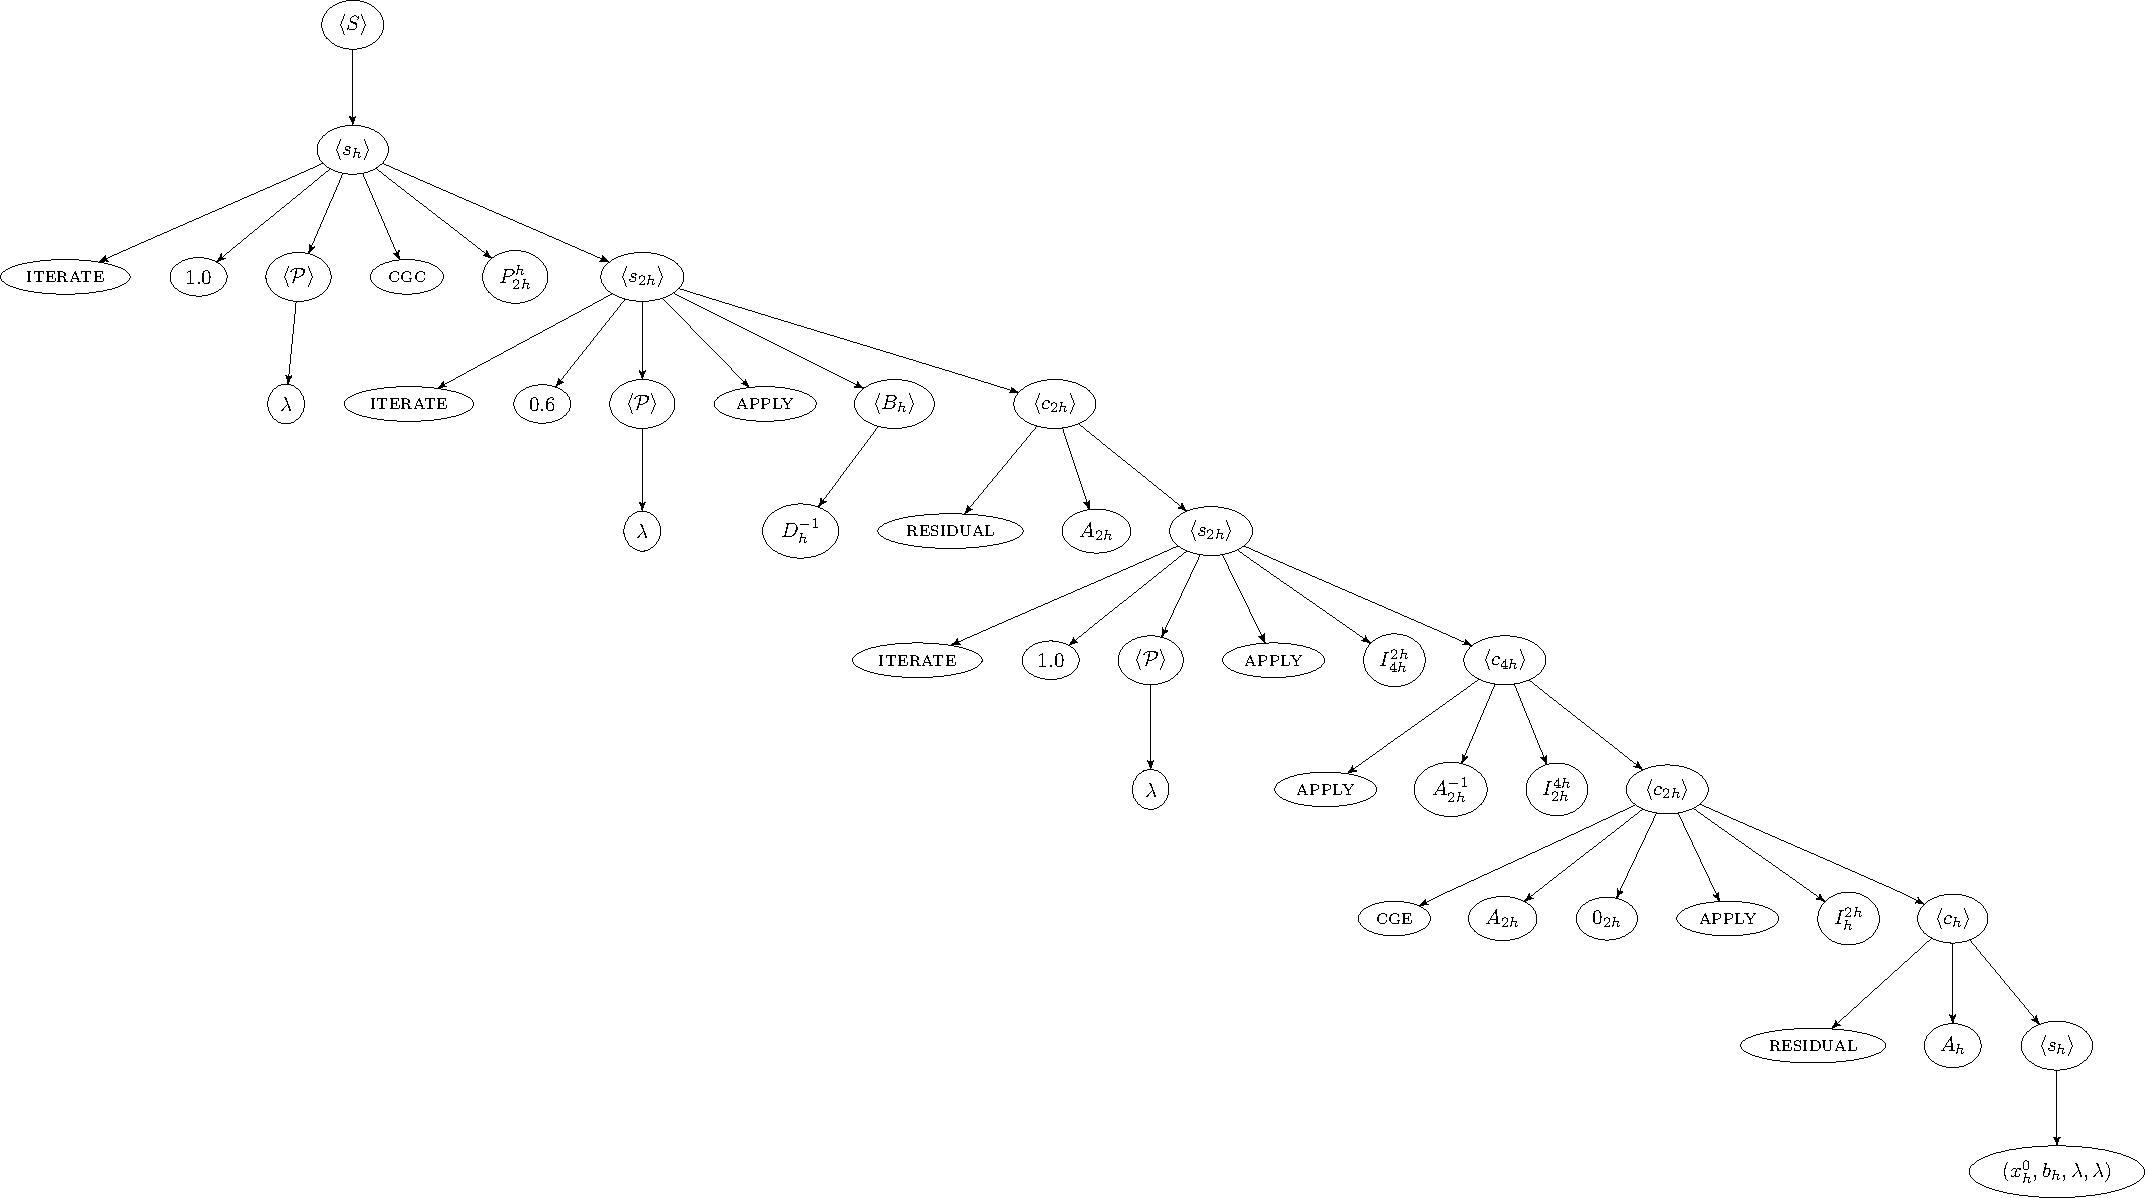
\includegraphics[width=\textwidth]{figures/trees/three_grid_method_grammar_tree.pdf}
	\caption{Grammar derivation tree for the three-grid method shown in Algorithm~\ref{alg:example-three-grid-method}.}
	\label{fig:example-three-grid-method-derivation-tree}
\end{figure}
Note that each inner node of the tree corresponds to a symbol that is contained in the set of variables $V$ of the grammar, as shown in Equation~\eqref{eq:multigrid-grammar-variables}, while all leaf nodes correspond to a terminal symbol.
As in the context of Algorithm~\ref{alg:multigrid-grammar} the application order of each function is well-defined, for the sake of simplicity, we have omitted all brackets in the tree.
%TODO evtl darauf eingehen, dass der CGS auf dem entsprechenden level spezifiziert sein muss
Until now we have been exclusively concerned with the problem of developing a formal representation for a multigrid method that is based on its algorithmic formulation, as for instance shown in Algorithm~\ref{alg:example-three-grid-method}, which can then be used to adapt each of its step individually, granting us the possibility to apply the grammar-based program optimization techniques presented in Section~\ref{sec:gggp}.
However, in contrast to Figure~\ref{fig:example-three-grid-method-derivation-tree} where we have started with an algorithmic representation, within grammar-guided genetic programming (GGGP) a derivation tree is usually \emph{grown} by applying a sequence of productions in a randomly-chosen order, either to alter an already existing tree or to create a completely new one from scratch.
We, therefore, have to consider the task of obtaining a method's algorithmic formulation exclusively based on its representation as a derivation tree and with respect to the semantic evaluation rules that apply to each of its nodes.
As we have seen in Section~\ref{sec:multigrid-state-transitions} the application of each of the functions that are generated by our grammar returns a new state $S_H$ consisting of a tuple $\left( \tilde{x}_{H}, b_{H}, c_{H}, S_{H/2}\right)$, where $H$ is the discretization width on the current level.
Starting from the initial state tuple $\left(x_{h}^0, b_{h}, \lambda, \lambda\right)$ we can, therefore, apply the respective transition functions in a bottom-up manner, until we arrive at the final state $\left(\tilde{x}_{h}, b_{h}, \lambda, \lambda\right)$.
As we have shown in Figure~\ref{fig:example-tree-grid-method-states} the first component $\tilde{x}_{h}$ of this tuple then combines all steps of the corresponding multigrid method in a single expression
\begin{multline}
	\tilde{x}_h = x_{h}^0 + I_{2h}^h ((0 + I_{4h}^{2h} A_{4h}^{-1} I_{2h}^{4h} (I_{h}^{2h}(b_{h} - A_h x_{h}^0) - A_{2h} 0)) + 0.6 \cdot D_{2h}^{-1} \cdot \\ 
	(I_{h}^{2h}(b_{h} - A_h x_{h}^0) - A_{2h} (0 + I_{4h}^{2h} A_{4h}^{-1} I_{2h}^{4h} (I_{h}^{2h}(b_{h} - A_h x_{h}^0) - A_{2h} 0)))).
	\label{eq:example-three-grid-method-expression}
\end{multline}
While this expression contains all necessary information about the computational structure of the method, certain terms occur multiple times, which might lead the redundant computations.
We can, however, remove this redundancy by considering Equation~\eqref{eq:example-three-grid-method-expression} as a computational graph, where each node either corresponds to an arithmetic operation or to a predefined symbol, such as $x^0_h$, $b_h$ and $A_h$.
The resulting graph for Equation~\eqref{eq:example-three-grid-method-expression} is shown in Figure~\ref{fig:example-three-grid-method-computational graph}.
\begin{figure}
	\centering
	\begin{subfigure}[b]{0.49\textwidth}
		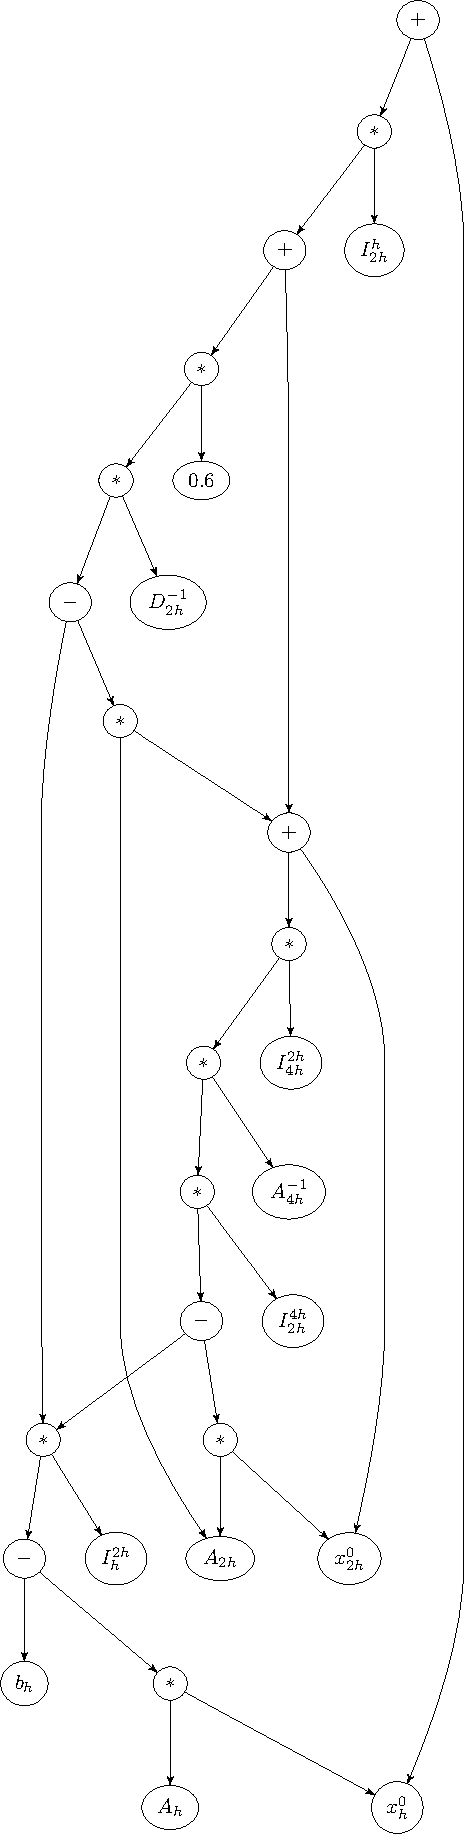
\includegraphics[scale=0.5]{figures/trees/three_grid_method_computational_graph.pdf}
		\caption{Computational graph for the three-grid method shown in Algorithm~\ref{alg:example-three-grid-method}.}
		\label{fig:example-three-grid-method-computational-graph}
	\end{subfigure}
	\centering
	\begin{subfigure}[b]{0.49\textwidth}
		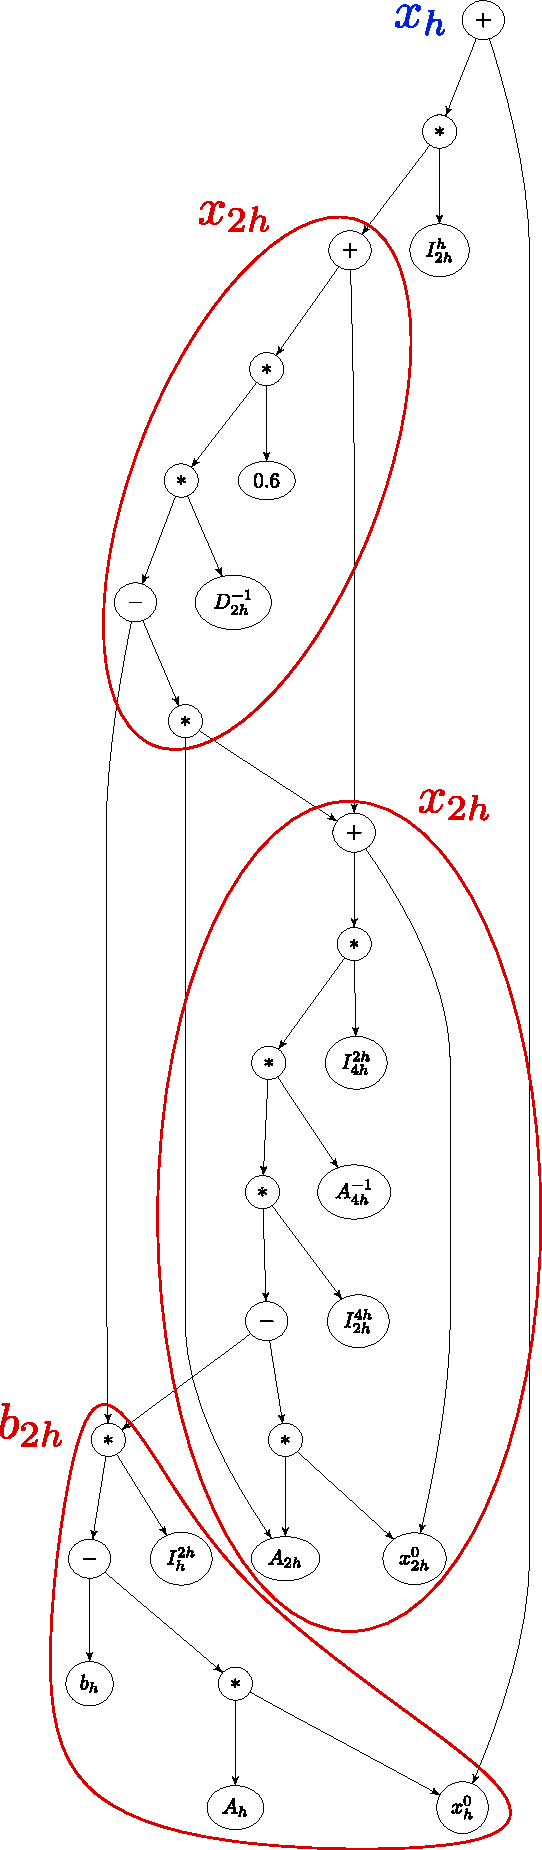
\includegraphics[scale=0.5]{figures/trees/three_grid_method_computational_graph_annotated.pdf}
		\caption{Assignment of subgraphs to the respective intermediate values.}
		\label{fig:example-three-grid-method-computational-graph-annotated}
	\end{subfigure}
\end{figure}
Again each node within this graph either corresponds to predefined symbol or an operation defined on vectors and matrices, whereby in case of the letter there exists a direct edge to each of the nodes that corresponds to one of its arguments.  
Therefore, whenever a certain node serves as an argument to more than one operations, multiple edges are directed towards it.
Based on this representation we can now define a redundancy-free sequence of computations that corresponds to the given multigrid method.
The most straightforward way to achieve this for a general graph is to simply introduce a temporary value for each non-leaf node of the graph.
However, note that each intermediate result in graph~\ref{fig:example-three-grid-method-computational-graph} that serves as an argument to multiple nodes either refers to a term representing the computation of an approximate solution or right-hand side on the respective level.
To verify this observation, consider again the three elementary multigrid operations listed in Definition~\ref{def:elementary-multigrid-operations}.
While a correction term is always discarded after its application, the current approximate solution is both needed in the construction of the current residual as well as whenever its value is updated, either through the application of smoothing or a coarse-grid correction.
Note that the same is true for the right-hand side, which is required whenever a new residual is constructed on a certain level.
This is illustrated in Figure~\ref{fig:example-three-grid-method-computational-graph-annotated}, where we have annotated all subgraph that correspond to the computation of an approximate solution or right-hand side.


 
